\documentclass[10pt,english,slidetop,compress,
              blue,mathserif,color=option]{beamer}
\usepackage[T1]{fontenc}
%\usepackage[latin9]{inputenc}
\PassOptionsToPackage{natbib=true}{biblatex}
\usepackage[style=authoryear]{biblatex}
%\usepackage{natbib}
%% Set how deep list environments go
\setcounter{secnumdepth}{3}
\setcounter{tocdepth}{3}

% Special link
\def\linkcomment{https://anu365-my.sharepoint.com/:b:/g/personal/u4166777_anu_edu_au/EeK_K1JK5xBEhnuH1ve4scQBebERBDPgNxMcK7s1sHJjUw?e=L9FW6m}

\usepackage{babel}
\usepackage{float}
\usepackage{booktabs}
\usepackage{amsmath}
\usepackage{amsthm}
\usepackage{amssymb}
\usepackage{graphicx}
\PassOptionsToPackage{normalem}{ulem}
\usepackage{ulem}

%% Legacy hack from other LyX generated tables
\providecommand{\tabularnewline}{\\}

%% Hyperlink stylin'
\ifx\hypersetup\undefined
  \AtBeginDocument{%
    \hypersetup{unicode=true,pdfusetitle,
 bookmarks=true,bookmarksnumbered=false,bookmarksopen=false,
 breaklinks=false,pdfborder={0 0 0},pdfborderstyle={},backref=slide,colorlinks=true,
 urlcolor=blue,linkcolor=blue,citecolor=red!20!brown!80!black}
  }
\else
  \hypersetup{unicode=true,pdfusetitle,
 bookmarks=true,bookmarksnumbered=false,bookmarksopen=false,
 breaklinks=false,pdfborder={0 0 0},pdfborderstyle={},backref=slide,colorlinks=true,
 urlcolor=blue,linkcolor=blue,citecolor=red!20!brown!80!black}
\fi

\makeatletter

%%%%%%%%%%%%%%%%%%%%%%%%%%%%%% Textclass specific LaTeX commands.
% this default might be overridden by plain title style
\newcommand\makebeamertitle{\frame{\maketitle}}%
% (ERT) argument for the TOC
\AtBeginDocument{%
  \let\origtableofcontents=\tableofcontents
  \def\tableofcontents{\@ifnextchar[{\origtableofcontents}{\gobbletableofcontents}}
  \def\gobbletableofcontents#1{\origtableofcontents}
}
\theoremstyle{plain}
\newtheorem{thm}{\protect\theoremname}
\theoremstyle{definition}
\newtheorem{defn}[thm]{\protect\definitionname}

%%%%%%%%%%%%%%%%%%%%%%%%%%%%%% User specified LaTeX commands.
%\usetheme{Warsaw}
%\usetheme{Boadilla}
\usepackage{threeparttable}
\usepackage{subfigure}
\usepackage{relsize}
\usepackage{url}
% Workaround for Linux: font library problem in Beamer
% See: https://tex.stackexchange.com/questions/383668/mktextfm-ecss0400-fails
\usepackage{lmodern}

\usetheme{default}
\useinnertheme[shadow]{rounded}
\usepackage{beamerinnerthemerounded}
% or ...
\usecolortheme{default}
% color themes: albatross, beaver, beetle, crane, default, dolphin, dov, fly, lily, orchid, rose, seagull, seahorse, sidebartab, structure, whale, wolverine

%\useoutertheme[subsection=false]{smoothbars}
% outer themes include default, infolines, miniframes, shadow, sidebar, smoothbars, smoothtree, split, tree

%\usecolortheme{orchid}
\setbeamertemplate{footline}[text line]{} % makes the footer EMPTY

\setbeamercovered{transparent}
% or whatever (possibly just delete it)

\usepackage{relsize}
\usepackage{tikz, tikzscale}
\usetikzlibrary{shapes,snakes}
\usetikzlibrary{calc}
\usepackage{relsize}
% Adapted from beamerinnerthemedfault.sty
\setbeamertemplate{itemize item}{\scriptsize\raise1.25pt\hbox{\donotcoloroutermaths$\blacktriangleright$}}
\setbeamertemplate{itemize subitem}{\tiny\raise1.5pt\hbox{\donotcoloroutermaths$\blacktriangleright$}}
\setbeamertemplate{itemize subsubitem}{\tiny\raise1.5pt\hbox{\donotcoloroutermaths$\blacktriangleright$}}
\setbeamertemplate{enumerate item}{\insertenumlabel.}
\setbeamertemplate{enumerate subitem}{\insertenumlabel.\insertsubenumlabel}
\setbeamertemplate{enumerate subsubitem}{\insertenumlabel.\insertsubenumlabel.\insertsubsubenumlabel}
\setbeamertemplate{enumerate mini template}{\insertenumlabel}
\setbeamersize{text margin left=20pt,text margin right=20pt}

\usefonttheme[onlymath]{structurebold}

%Color scheme - TK modified
%\setbeamercolor{normal text}{fg=brown!20!black,bg=brown!50!white}
%\setbeamercolor{title}{fg=red!50!black}xxxx
%\setbeamercolor{section in head/foot}{fg=red!40!black,bg=white!80!brown}
%\setbeamercolor{frametitle}{fg=brown!60!orange!50!black}
\setbeamercolor{item}{fg=orange!50!yellow!80!red!20!blue!20!black}  %{fg=orange!50!red!50!brown}
\setbeamercolor{math text}{fg=blue!90!green!60!black} %{fg=brown!50!red!60!black}
\setbeamercolor{alerted text}{fg=red!30!black!60!brown}
\setbeamercolor{quote}{fg=blue!90!green!60!black}
\setbeamercolor{block title}{fg=red!40!black!60!brown}
\setbeamercovered{transparent=25}
\setbeamercolor{button}{fg=orange, bg=gray!30!white}

\makeatletter
\define@key{beamerframe}{wide}[30pt]{%
  \def\beamer@cramped{\itemsep #1\topsep0.5pt\relax}}
\makeatother

%gets rid of bottom navigation bars
\setbeamertemplate{footline}[21]{}

%gets rid of bottom navigation symbols
\setbeamertemplate{navigation symbols}{}

%gets rid of footer
%will override 'frame number' instruction above
%comment out to revert to previous/default definitions
\setbeamertemplate{footline}{}

\makeatother

% Color settings - custom defs
\usepackage{color}
\definecolor{sangre}{rgb}{0.6,0.18,0.19}
\definecolor{dullmagenta}{rgb}{0.4,0,0.4}
\definecolor{darkblueroyale}{rgb}{0,0,0.6}
\definecolor{verdeprofundo}{rgb}{0.02,0.376,0.031}
\definecolor{aqua}{rgb}{0.0, 1.0, 1.0}


\providecommand{\definitionname}{Definition}
\providecommand{\theoremname}{Theorem}

%% ============================================================================
%%    CUSTOMIZABLE: Title Page Information
%% ----------------------------------------------------------------------------
\title[]{Monetary Policy Transmission in Sri Lanka}

\author[        ]{          
  Theseem Muhammadu Theseem {\color{gray}(University of Wollongong)} 
                      \\
                      -
                      \\
                       Discussant: Timothy Kam {\color{gray}(ANU/SKKU)}
                      }

%\institute[~QED-ANU/RSE]{
%                    \color{gray!50!black}
%                    \inst{1}Monash University
%                    \\
%                    %\and
%                    \inst{2}Australian National University
%                    }

\date{ \color{gray!80!blue}

      {\smaller PhD Conference, Nov 11-12, 2021}
      \\
      \bigskip
      
}

\addbibresource{references.bib}




\begin{document}
%% ============================================================================
\begin{frame}
  \titlepage
\end{frame}



%% ==========================================================================
%%      MILESTONE SLIDE - 
%% ==========================================================================
{
\setbeamercolor{background canvas}{bg=gray!40!black}
  \begin{frame}
    \begin{center}
      \bigskip
      \bigskip
      {\Huge\bfseries{\color{orange}What do the authors do?}}
      \bigskip

    \end{center}
  \end{frame}
}

%% ============================================================================
\begin{frame}{What do the authors do?}

  Authors raise the following questions:
  \bigskip

  \begin{enumerate}
    \item Effect of monetary policy (\textbf{MP}) on Sri Lanka's real economy?
    \begin{itemize}
      \item Importance of \textbf{Cr}edit and \textbf{Ex}change-rate channels in \textbf{MP} tranmission?
    \end{itemize}

    \bigskip

    \item What are the changes in \textbf{MP} Transmission Mechanism post civil war?
    
    \bigskip

  \item How do credit shocks affect the economy?
  \end{enumerate}

\end{frame}

%% ============================================================================
\begin{frame}{What do the authors do?}
  \begin{enumerate}
    % \item Authors study Sri Lanka's macroconomy from a VAR lens.
    \item Growth-rate of key variables (*except): 
      \begin{itemize}
        \item \textbf{O}il \textbf{P}rice, 
        \item \textbf{F}ed \textbf{F}unds \textbf{R}ate, 
        \item \textbf{F}orex \textbf{E}xchange \textbf{R}eserves, 
        \item \textbf{Y} real GDP,
        \item \textbf{INF}lation (CPI),*
        \item \textbf{M1},
        \item \textbf{INT}erest rate (money market)*
        \item \textbf{CR}edit to private sector from commercial banks,
        \item \textbf{R}eal \textbf{E}xchange \textbf{R}ate.*
      \end{itemize}
    \item VAR($p$), $p=2$, linear trend, constant, peace dummy (mid 2009--).
    \item Data: 1996-Q1 to 2019-Q4.
    \item Study \textbf{MP} transmission:
      \begin{itemize}
        \item Identify ``structural'' shocks assuming Cholesky factorization---variables ordered above.
        \item Estimated impulse response function (IRF) and variance decomposition (VD) statistics.
      \end{itemize}
  \end{enumerate}
\end{frame}



%% ============================================================================
\begin{frame}{Contribution and Claimed insights}

  Interesting question: Pre-/post-war nature of MP transmission. Has MP become better?

  \begin{enumerate}
    \item (\textbf{MP}) has ``expected'' dynamic multiplier effects on real economy. Importance of \textbf{Cr}edit and \textbf{Ex}change-rate channels in \textbf{MP} tranmission.
    
    \bigskip

    \item Post civil war effect of (\textbf{MP}) has stronger and more persistent effect on the economy. (Implies ``better'' MP effects?)
    
    \bigskip

  \item Increased bank lending raises output and inflation.
  \end{enumerate}
  
\end{frame}

%% ==========================================================================
%%      MILESTONE SLIDE - 
%% ==========================================================================
{
\setbeamercolor{background canvas}{bg=gray!40!black}
  \begin{frame}
    \begin{center}
      \bigskip
      \bigskip
      {\Huge\bfseries{\color{orange}Specific Comments/Suggestions}}
      \bigskip

    \end{center}
  \end{frame}
}


%% ============================================================================
\begin{frame}{Comment 1: MP shock and transmission}

  \begin{enumerate}
    \item What is the monetary policy (instrument) said to be identified in the VAR?
    \begin{itemize}
        \item Nowhere defined/discussed in the paper. Turns out to be \textbf{INT} (money-market interest rate). Reader inferred from Figure 1 (impulse responses).
        
        \item Problem is that Figure 1 impulse responses are mostly ``insignificant'' (not statistically different from zero). Exception: output, M1, RER.
        
        \item Are these IRF bands asymptotic bands? Tried boostrapping these given small-sample size problem?
      \end{itemize}

    \item Claimed: \textbf{CR} and \textbf{RER} have more persistent responses to MP shock imply that the ``credit'' and ``exchange-rate'' channels are important to MP. Why? If anything, the rest of the variables do not respond to MP shock $\Rightarrow$ MP is not effective in stimulating the domestic economy?

    
  \end{enumerate}

\end{frame}

%% ============================================================================
\begin{frame}{MP shock and transmission}
  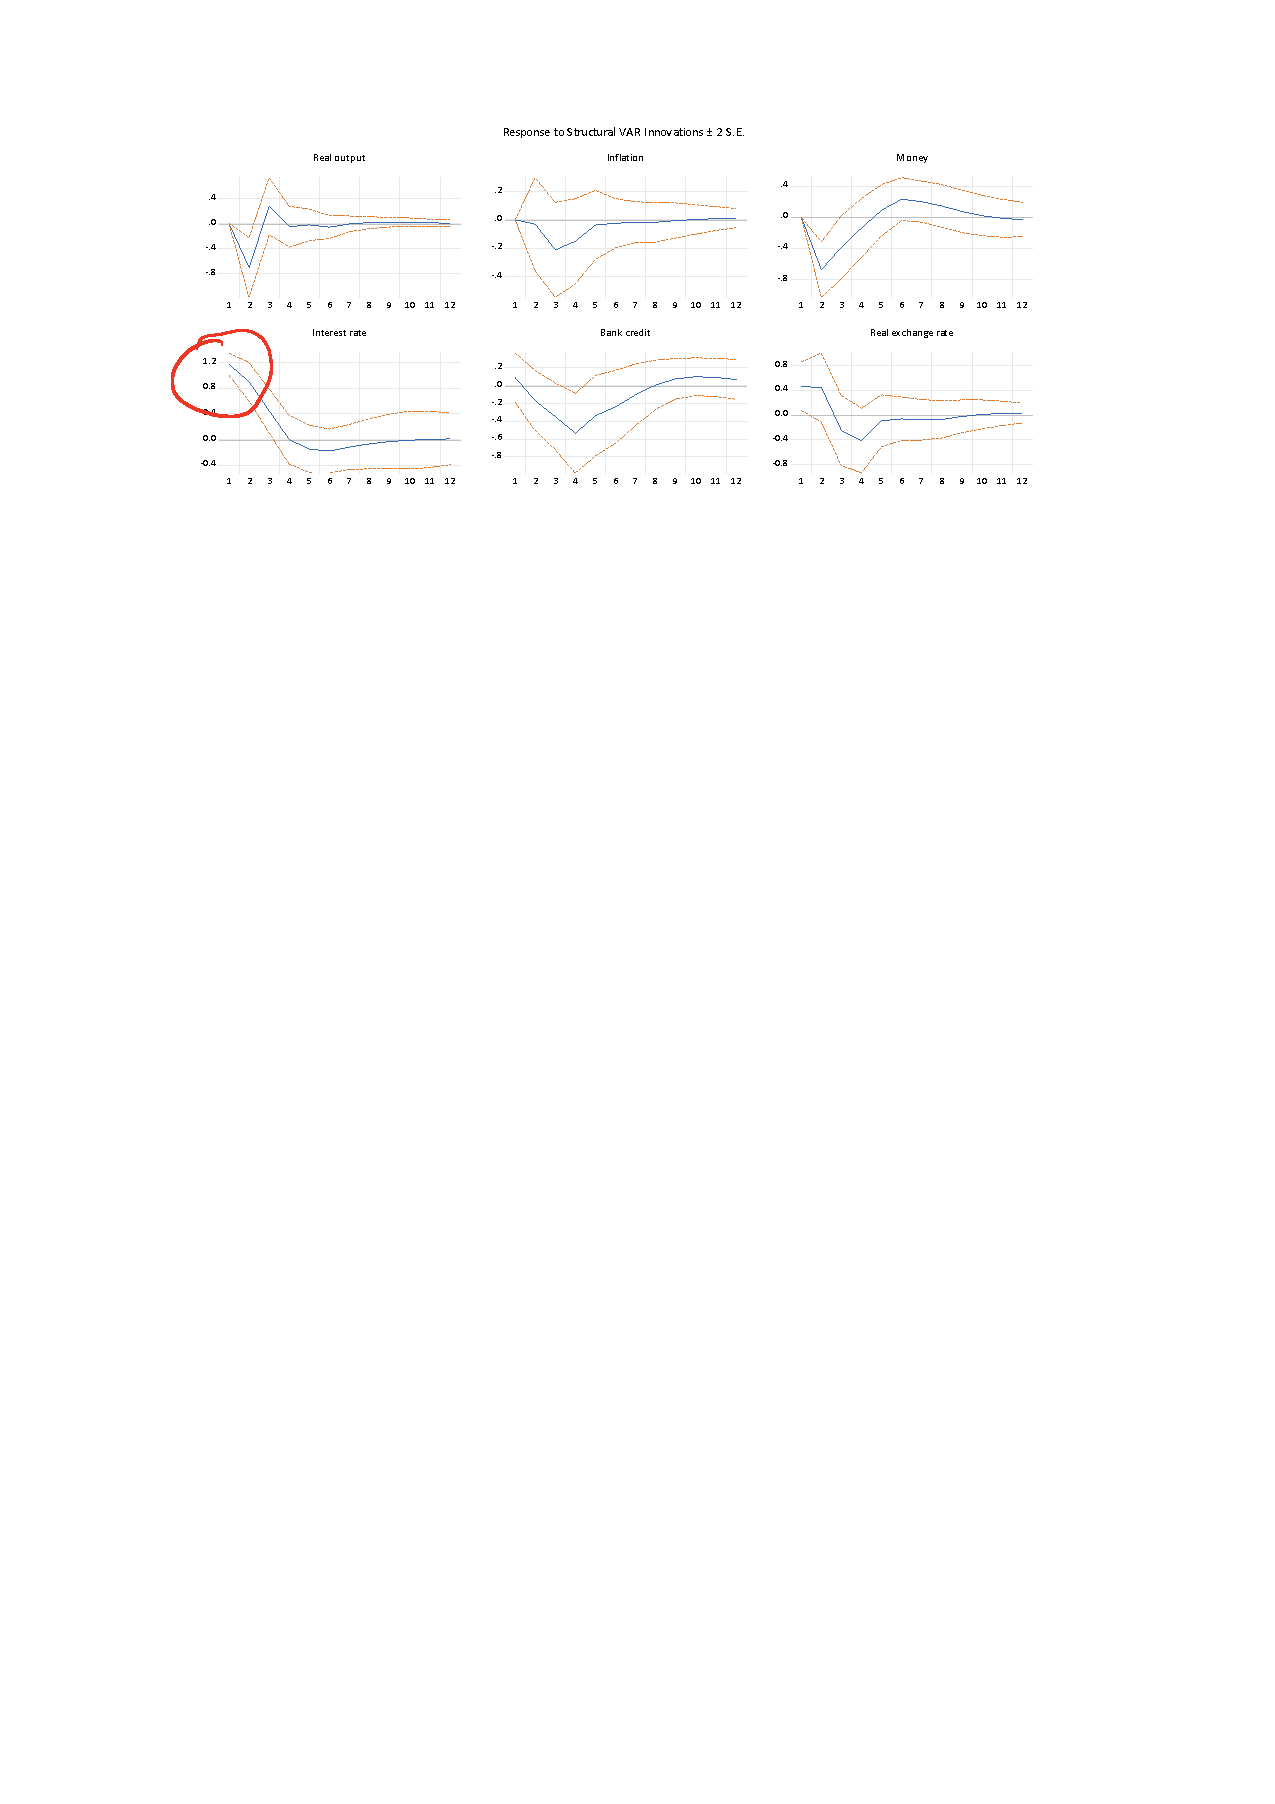
\includegraphics[width=0.99\textwidth]{figures/MP-shock.pdf}
\end{frame}


%% ============================================================================
\begin{frame}{Comment 2: Pre-/post-war MP transmission}

  Post war: IRFs (given MP shock) decay slower and have larger magnitudes.
    \begin{itemize}
      \item Relative pre-/post-war comparison limited to Table 2 (point estimates).
      \item Suggest to plot these. Also show IRF error bands!
    \end{itemize}  

  Stronger post-war effect of MP shock:
    \begin{itemize}
      \item Is this somehow related CBSL's declining ability to defend its currency? See figures next ... 
      \item Would be interesting if authors can pursue this and tell us more: how and why.
    \end{itemize}

\end{frame}

%% ============================================================================
\begin{frame}{An FER story? How?}
  \framesubtitle{Drastic jumps and volatility circa/post 2009}
  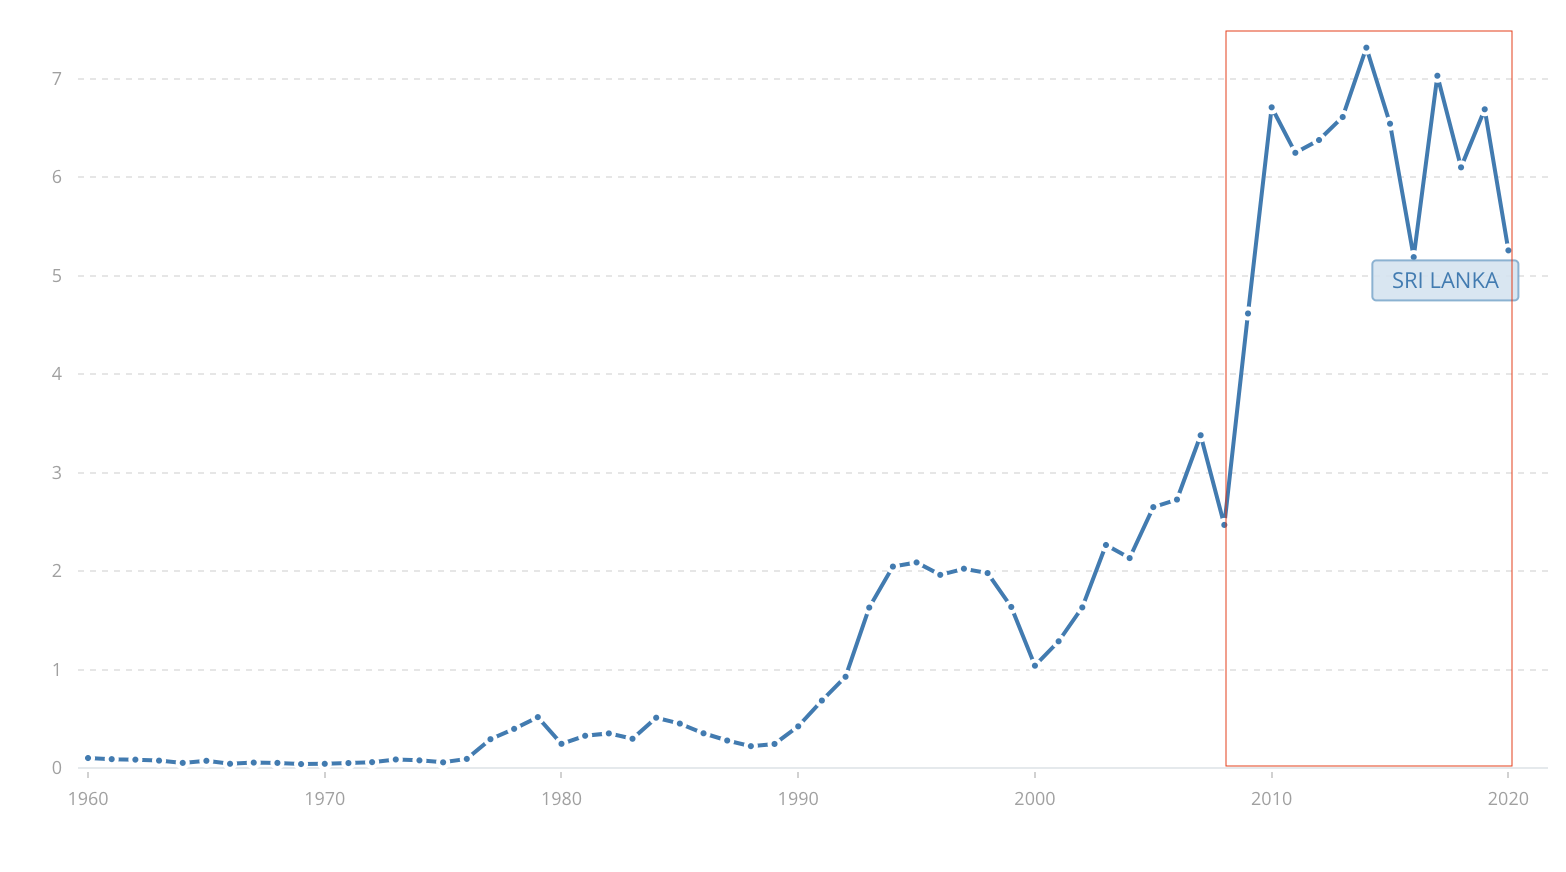
\includegraphics[width=0.95\textwidth]{figures/total-reserves-exgold.png}
  \begin{center}
    Total Reserves (minus gold)
  \end{center}
\end{frame}

\begin{frame}{An FER story? How?}
  \framesubtitle{
    Declining ability to defend currency and/or rising debt burden?
    }
  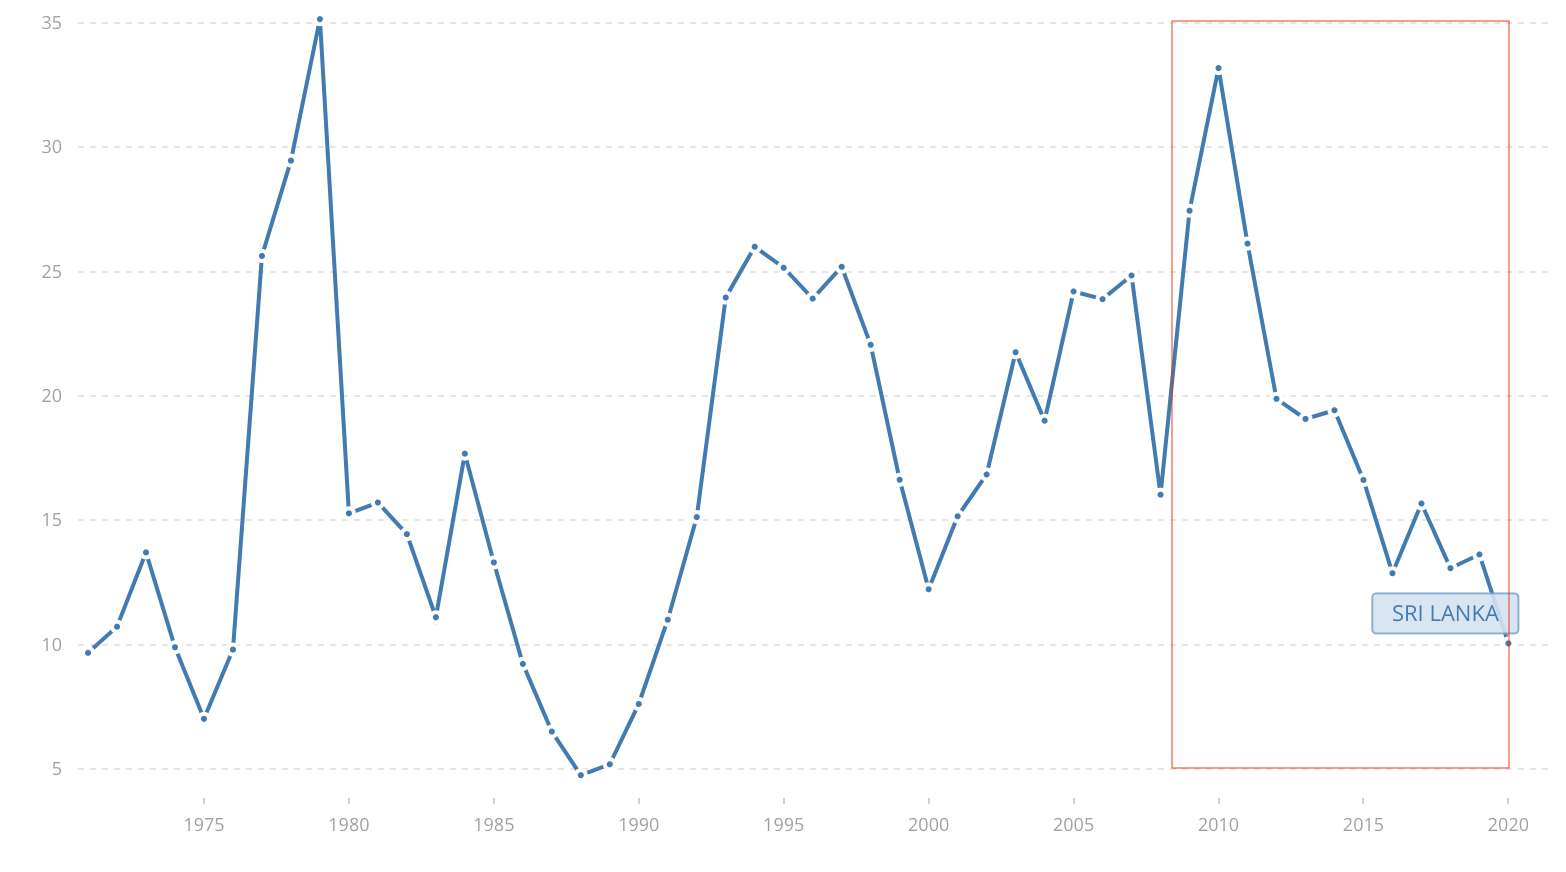
\includegraphics[width=0.95\textwidth]{figures/total-reserves-to-external-debt.png}
    \begin{center}
      Total Reserves / External Debt ratio
    \end{center}
\end{frame}

\begin{frame}{An FER story? How?}
  \framesubtitle{Post 2009: CBSL's rising liability against FER asset ...}
  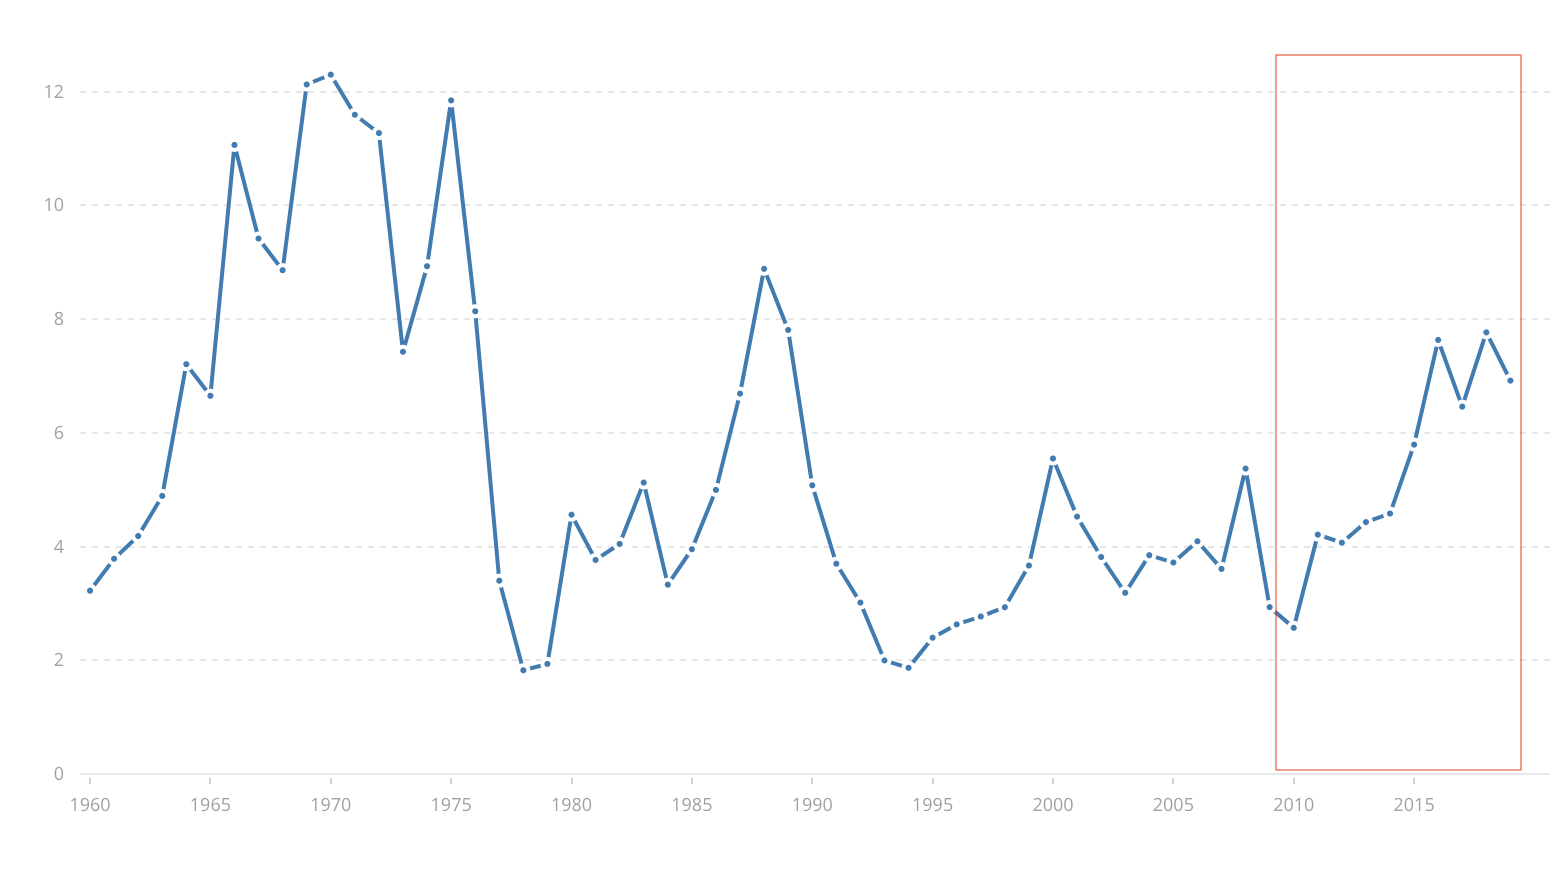
\includegraphics[width=0.95\textwidth]{figures/M0-to-totalreserves.png} 
  \begin{center}
    MO / Total Reserves
  \end{center}
\end{frame}

\begin{frame}{Comment 2: An FER story? How?}
  From CBSL's operations and news commentaries, CBSL official interest-rate corridor policy seems to be tempered by \textbf{FER} (forex reserves management).

  \bigskip
  Suggestion: Focus on this aspect of policy?
    \begin{itemize}
      \item 
      \item How to separately identify structural \textbf{INT} variations in the presence of potential \textbf{FER} management?
      \item Is merely ``chucking'' in \textbf{FER} sufficient for identifying policy variations hidden in observed \textbf{INT} outcomes?
      \item Given current setup ... Suggestion: Order \textbf{FER} then \textbf{INT} lowest in the "triangle"?
    \end{itemize}
\end{frame}


%% ============================================================================
\begin{frame}{Comment 3: "Credit channel"}

  Positive shock to lending (\textbf{CR})
    \begin{itemize}
        \item Claimed: raises output and inflation
        \item Comment: But all these IRFs are statistically no different from zero.
        \item What really is ``credit channel''? Is a shock to \textbf{CR} a supply-side (lender) or a demand-side shock? Here, it seems to be both since \textbf{CR} only measures observed lending and borrowing. Do they have different MP implications? If so, do we need to separately identify a lending-side shock in line with authors' intention?
        \item Suggestion: 
        \begin{itemize}
          \item Is modelling the economy in a growth-rates VAR appropriate? E.g., a shock to \textbf{INT} would actually be a shock to the \emph{acceleration} of monetary policy rate. 
          \item Have authors tried a VECM with mixture of I(0) and I(1) variables? \citet{phillips1995}; \citet{chang-phillips1995}.
        \end{itemize}
    \end{itemize}  
\end{frame}

%% ============================================================================
\begin{frame}{"Credit channel"}
  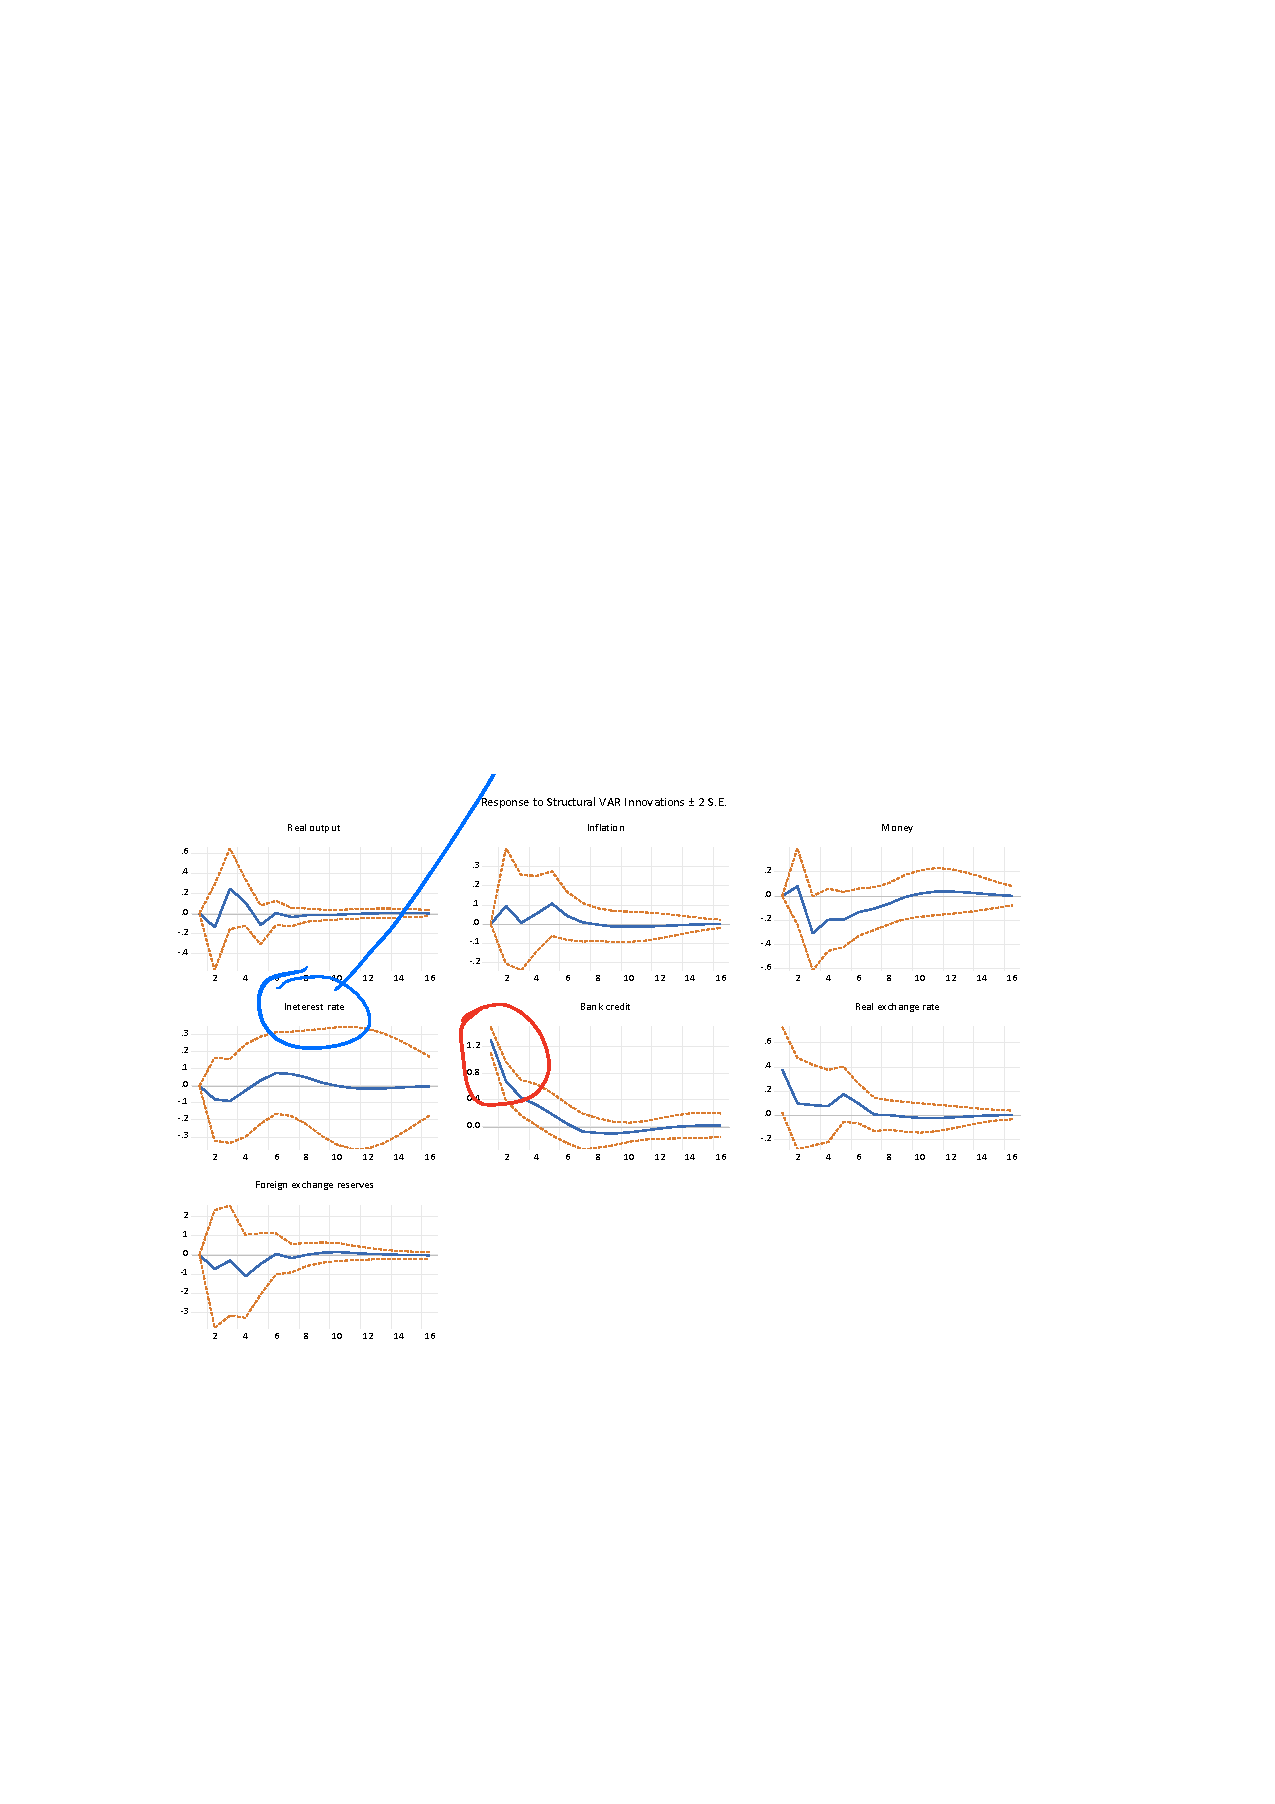
\includegraphics[width=0.99\textwidth]{figures/CR-shock.pdf}
\end{frame}

%% ============================================================================
\begin{frame}{Comment 4: Real trade sector?}
  
  Sri Lanka has been heavily dependant on tourism, trade and FDI. 
  \bigskip

  Suggest to include
  \begin{itemize}
    \item FDI
    \item Current/capital account elements
  \end{itemize}

\end{frame}

%% ============================================================================
\begin{frame}{Comment 5: Miscellany}
  Please check:
  \begin{itemize}
    \item Spelling
    \item Punctuation
    \item Long sentences
    \item Footnoting convention
    \item Make growth-rate variables notation more obvious?
    \item Report lag-length selection criteria?
    \item Report estimation method: OLS, software. Replicable science!
    \item Consistency of citation style
  \end{itemize}

  Detailed \href{\linkcomment}{notes/comments here}.
\end{frame}


% ==========================================================================
%%      BIBTEX REFERENCING OUTPUT
%% ==========================================================================
% \begin{frame}[allowframebreaks]{References}
%   \begin{smaller}
%     \printbibliography
%     %\thebibliography{bjbanks}
%   \end{smaller}
% \end{frame}

% ==========================================================================
%%      BIBTEX REFERENCING OUTPUT
%% ==========================================================================
\begin{frame}{References}
  \begin{smaller}
    \printbibliography
    %\thebibliography{bjbanks}
  \end{smaller}
\end{frame}



\end{document}
